The mission outline is separated in five phases: Launch, interplanetary transfer, aerocapture and entry, terminal descent and return. The design of the \gls{cia} is focussed on the aerocapture and entry phase. %All of these mission phases are discussed in the subsequent Sections.

\subsubsection{Launch} \label{sec:launch}
Mission launch is the first phase of the mission. Launch serves to bring the \gls{hiad} and accompanying mission elements in a transfer orbit towards Mars. From the top level requirements as summarised in \ref{sec:missionreq} an approach speed of 7 [$km\cdot s^{-1}$] is desired which is an implicit requirement on the total mission duration.
Based on this requirement specific launch operations can be considered and additional mission requirements can be considered. Important factors include payload size, loads and required velocity increments. Launch is important to consider also in the \gls{hiad} design as a lot of the requirements can be traced down to mission launch.

The launch mission phase initiates with the take-off from earth. In order to reach the Martian atmosphere with the desired approach speed a total velocity increment of about 19.6 [$km\cdot s^{-1}$] is required. This velocity increment comes forth of the escape velocity of the Earth to its sphere of influence and an additional velocity increment to reach the Martian atmosphere with the required approach velocity.

The velocity increments are typically subdivided into two parts: a first velocity increment into \gls{leo} and a second velocity increment into the transfer orbit. Within the \gls{leo} separate payload modules such as the \gls{hiad} and a possible habitation module may be joined \cite{George2009}. The period in \gls{leo} also allows for more precisely controlled arrival conditions at Mars as, to a certain extend, the launch is omitted from the timing sequence. 

The velocity increments up to \gls{leo} are typically subdivided into multiple integrated stages or launchers for optimal efficiency as no single launcher can deliver the total required velocity increment. These stages are separated after depletion of the propellant.

Important considerations concerning the launch are the encountered vibrations and loads as well as the total mass required to bring into the transfer orbit. Launch vibration should be considered as the natural frequencies of the subsystem should remain above the launch-induced vibrations. Moreover the vibrations require all components to be properly stowed. This should for example be considered for the inflatable part of the decelerator, which is stowed during launch.

Launch loads are typically in the order of 2.8-4.3 g's in longitudinal and 0.9-3 g's in lateral direction \cite{Wertz2011}, which is above the maximum allowed top level deceleration of 3g into the Martian atmosphere. For this reason launch loads are an important factor for the structural sizing of the aeroshell and accompanying elements. 

A launcher currently being developed for missions to Mars is the \acrfull{sls} developed by \gls{nasa}. The \gls{sls} features multiple stages and allows for a 5 [$m$] diameter in line with the top level mission requirements. The \gls{sls} features multiple stages able to deliver the required velocity increments. Its design takes close account of the Orion spacecraft which is being developed to, in the future, go to Mars. For the modules featuring a 5 [$m$] diameter payload the volume using this launcher is constraint to 225 [$m^3$] \cite{NASA2014}.

The launch phase is concluded with the start of the interplanetary phase after the final velocity increment in \gls{leo}. 



\subsubsection{Interplanetary transfer} \label{sec:interplanetary}
The interplanetary transfer time has a big impact on the design. The interplanetary transfer time determines for instance the mass of food for the astronauts, the amount of radiation to endure, how much they need to exercise and more. Keeping the transfer time short will minimise these problems. However it will also increase the $\Delta\gls{sym:V}$-budget needed for the launcher. 

\begin{figure}[h]
	\centering
	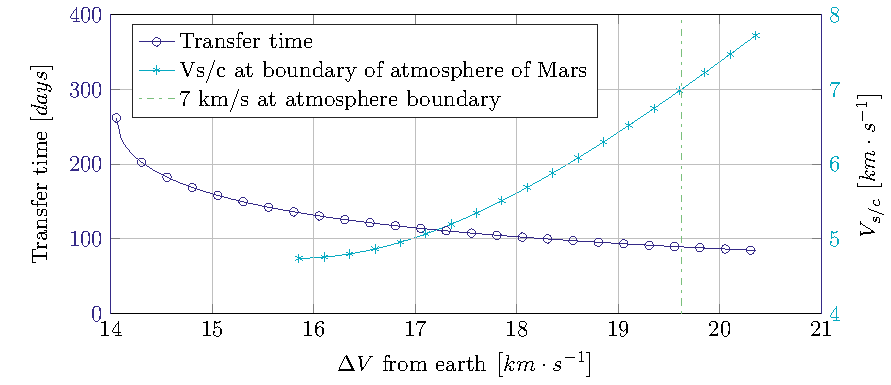
\includegraphics[width=0.95\textwidth]{Figure/Inter_transfer/transfer_time.pdf}
	\caption[Interplanetary transfer time and entry velocity versus $\Delta\gls{sym:V}$]{Interplanetary transfer time (left) and entry velocity (right) versus $\Delta\gls{sym:V}$}
	\label{fig:inter_time}
\end{figure}

The most efficient transfer with respect to the $\Delta\gls{sym:V}$-budget consists of a Hohmann transfer orbit. This would take approximately 262 days. This time is the longest of all orbits to Mars with a direct transfer. One of the mission requirements is the entry velocity of $7 \left[km \cdot s^{-1}\right]$. This velocity is fully determined by the $\Delta \gls{sym:V}$ budget and thereby corresponds to the transfer time. In Figure \ref{fig:inter_time} this relation is visualised. As can be seen to arrive with the required velocity a $\Delta \gls{sym:V}$ of $19.62 \left[km \cdot s^{-1}\right]$ is required, which corresponds to a transfer time of $89.3$ days. The corresponding orbit is shown in Figure \ref{fig:inter_orbit}.

\begin{figure}[h]
	\centering
	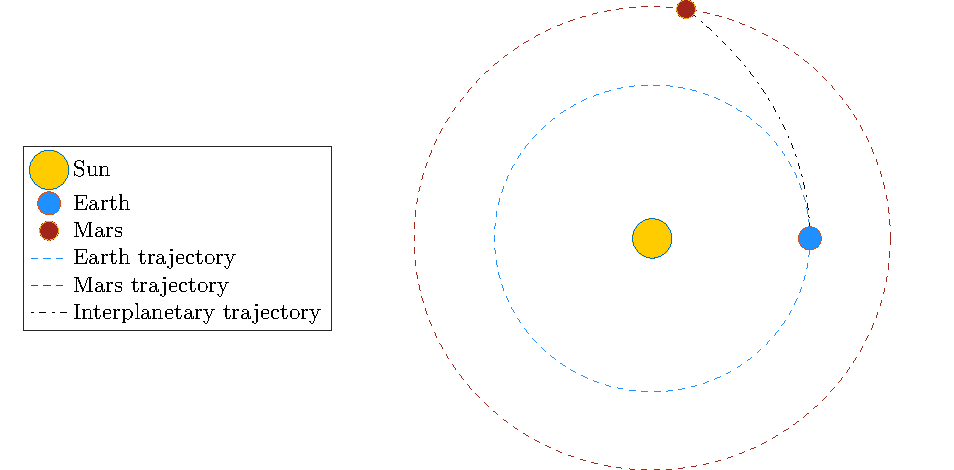
\includegraphics[width=0.95\textwidth]{Figure/Inter_transfer/orbits.pdf}
	\caption[Visualisation of the interplanetary transfer orbit]{Visualisation of the interplanetary transfer orbit. Planets not to scale}
	\label{fig:inter_orbit}
\end{figure}


\subsubsection{Aerocapture and entry} \label{sec:entry}
The third phase of the mission is the arrival at Mars and the deceleration to a velocity of $M=5$ at $15$ $\left[km\right]$ height above the surface of Mars with an accuracy of $500 \left[m\right]$ in each direction. This deceleration is split into an initial aerocapture, a parking orbit and a final entry. The combined sum of these components should not take longer than 10 Earth days. In this phase of the mission the \gls{hiad} is used to decelerate the capsule and protect it against the thermal loads imposed by the deceleration. In addition, taxation of human crew members requires loads not to exceed 3\gls{con:ge}.

%Upon arrival on Mars, first the interplanetary habitat is separated from the entry capsule. The habitat will be put on a trajectory which causes it to burn up in the vicinity of the sun.
Upon arrival at Mars the first thing that happens, just before the spacecraft enters the atmosphere, is the deployment and inflation of the \gls{hiad}. %The aeroshell will be continuously kept at pressure during the rest of the mission phase.
%The spacecraft is now transformed into a entry vehicle and is ready to start the aerocapture.

The entry vehicle then enters the atmosphere for the first time. This first pass through the atmosphere is called aerocapture. The entry vehicle will fly through the atmosphere following a pre-determined path using active bank control. A real-time controller will manage the active control systems to account for unexpected differences in atmospheric properties. The goal of this controller is to keep the kinetic energy lost during the aerocapture equal to what is pre-calculated. This loss of kinetic energy determines the characteristics of the trajectory which the spacecraft will follow once it leaves the atmosphere. %Diminishing too little energy causes the trajectory to be more eliptic or even hyperbolic. Diminishing too much energy causes the the trajectory to be less eliptic, or it can even cause the entry vehicle to not even go out of the atmosphere anymore. These trajectory characteristics change the orbit period and the fuel fraction needed to change 

After the aerocapture the spacecraft goes into an elliptic Kepler orbit. When the spacecraft is headed to the apocentre of the orbit it changes attitude so that the thrusters point in the along-path direction to give the spacecraft a velocity change. While in the apocentre the spacecraft gets a $\Delta\gls{sym:V}$ to raise the pericentre altitude of the Mars-centred orbit to a parking orbit at 200 $[km]$ height.
%In the apocentre the spacecraft gets a velocity change which will get it in an elliptic Mars-synchronous orbit which will not pass through the atmosphere. 

From this parking orbit the atmospheric conditions can be observed and a plan can be made for the entry into the atmosphere in order to get to the intended landing location. The observations made of the atmosphere will help determine a suitable moment to do the final entry and will give information that can be used to predict the final entry trajectory more accurately. For example, in case of a dust storm, characteristic of Mars, \gls{edl} can be delayed until it has passed.

Once the decision has been made to conduct the final entry the spacecraft is given a second boost to decelerate it just enough to get the entry vehicle into the desired trajectory. Here, just as during the first pass through the atmosphere, the spacecraft is controlled using active bank control managed by a real-time controller. %When the entry vehicle is approaching the intended final location at $10 \left[km\right]$ height a change in angle of attack is used to dive to that location. Having control over the time of initiation of the dive gives us an additional safety on landing within  $500 \left[m\right]$ from the target.

\subsubsection{Terminal descent} \label{sec:terminal}
The terminal descent of the spacecraft is the part of the mission between the end of aerocapture and landing on the surface of Mars. The velocity is to be brought back to zero at an altitude of zero, from an initial velocity at the end of the aerocapture phase of the mission. For the terminal descent, several design options are available to decrease the velocity. In this section, firstly, the mission characteristics are discussed. After that, the design options are summarized after which a choice is made based on feasibility and performance.

\paragraph{Terminal descent characteristics}
The start of this part of the mission is given by the end of the aerocapture part, of which the requirements dictate a Mach number of $5$ at a height of $15$ [km], as given in Section \ref{sec:missionreq}. This means the aerodynamic flow regime changes from hypersonic to supersonic, and finally to subsonic during the terminal descent. The speed of sound in the lowest fifteen kilometres of Mars is approximately $220$ $[m\cdot s^{-1}]$, which means the velocity of the spacecraft is $1100$ $[m\cdot s^{-1}]$ at the beginning of terminal descent. The velocity only marginally increases due to the gravity influence of Mars: the velocity with no deceleration would be 3 percent higher on the surface of Mars than at an altitude of $10$ $[km]$, assuming no deceleration due to drag or thrust. Finally, the flight path angle is not predetermined by the orbit, so it can be changed to fit the needs of the terminal descent phase.

\paragraph{Design options}
Terminal descent can be split up in two parts: the supersonic and subsonic flight part and final touchdown. For both parts, different options are available.

The first option for the flight is to use retro-propulsion for every part of the descent. The fuel mass would be about $23.3\%$ of the total spacecraft mass if no aerodynamic effects were taken into account. However, the aeroshell has a large frontal area which adds a significant amount of drag. Also, in numerical simulations and wind tunnel tests the interaction between retro-propulsion and the aeroshell were found to result in a mass fraction that is approximately twice as small as would be expected when considering the thrust and drag forces to act independently of each other \cite{Korzun2009}. Since a blunt body is unstable at transonic and supersonic speeds, a small drogue parachute is needed to stabilise the spacecraft. Scaling a mass estimate for an inflatable aeroshell from NASA, this stabilisation drogue parachute is approximately 20 [kg] including 20$\%$ contingency.
The fuel mass is estimated assuming a constant deceleration of 3 [\gls{sym:ge}]. This condition in combination with the initial conditions of the terminal descent, leads to a specified flight path angle of 38 [deg] and a velocity at each height. Using this velocity, the drag was calculated assuming the same drag coefficient throughout the supersonic regime. This analysis is known to be incorrect to a certain level, but since it is preliminary analysis this is taken for granted. The drag at every height leads to a deceleration lower than 3 [\gls{sym:ge}], and thrust is delivered at a level such that this deceleration is achieved, incorporating the gravitational force. The drag, thrust and total required force are plotted in Figure \ref{fig:TDforce}. This requires the rocket engines to be sized such that, a total thrust of 312 [kN] is achieved. To this end, 3 RL 10A-4 rocket engines are placed at the front of the centerbody. The mass of these rockets is 504 [kg] combined. The thruster fuel flow is calculated using the specific impulse of the engine, 451 [s], and integrated over time to find the total fuel, estimated to be 680 [kg] \cite{Wertz2011}. The tank mass is estimated using an empirical relation, at 45 [kg] and assuming a density of 1 $[kg\cdot dm^{-3}]$ for the fuel \cite{Wertz2011}.

\begin{figure}
	\centering
	\setlength\figureheight{0.4\textwidth} 
	\setlength\figurewidth{0.7\textwidth}
	% This file was created by matlab2tikz.
% Minimal pgfplots version: 1.3
%
\definecolor{mycolor1}{rgb}{0.00000,0.44700,0.74100}%
\definecolor{mycolor2}{rgb}{0.85000,0.32500,0.09800}%
\definecolor{mycolor3}{rgb}{0.92900,0.69400,0.12500}%
%
\begin{tikzpicture}

\begin{axis}[%
width=0.95092\figurewidth,
height=\figureheight,
at={(0\figurewidth,0\figureheight)},
scale only axis,
xmin=0,
xmax=36.2,
xlabel={$t [s]$},
xmajorgrids,
ymin=0,
ymax=327.127499399344,
ylabel={$F [kN]$},
ymajorgrids,
axis x line*=bottom,
axis y line*=left,
legend style={at={(0.97,0.5)},anchor=east,legend cell align=left,align=left,draw=white!15!black}
]
\addplot [color=mycolor1,solid,mark=o,mark options={solid}]
  table[row sep=crcr]{%
0	311.243849696306\\
3	311.2690765018\\
6	311.294330905114\\
9	311.31961294652\\
12	311.344922666362\\
15	311.370260105056\\
18	311.395625303094\\
21	311.421018301041\\
24	311.446439139536\\
27	311.471887859293\\
30	311.4973645011\\
33	311.52286910582\\
36	311.548401714389\\
};
\addlegendentry{Required force};

\addplot [color=mycolor2,solid,mark=diamond,mark options={solid}]
  table[row sep=crcr]{%
0	291.174450058233\\
3	277.302732528785\\
6	258.852292042653\\
9	236.781994493662\\
12	211.655388803588\\
15	182.707467963119\\
18	150.782315705625\\
21	118.023689876921\\
24	85.8538439967556\\
27	55.3620239309924\\
30	28.4892892980397\\
33	8.59563822808\\
36	0.0416064994811875\\
};
\addlegendentry{Drag};

\addplot [color=mycolor3,solid,mark=square,mark options={solid}]
  table[row sep=crcr]{%
0	20.0693996380731\\
3	33.9663439730147\\
6	52.442038862461\\
9	74.5376184528585\\
12	99.6895338627736\\
15	128.662792141937\\
18	160.613309597469\\
21	193.397328424119\\
24	225.59259514278\\
27	256.109863928301\\
30	283.00807520306\\
33	302.927230877739\\
36	311.506795214908\\
};
\addlegendentry{Thrust};

\end{axis}
\end{tikzpicture}%
	\caption{Thrust, drag and required force for 3 [\gls{sym:ge}] deceleration starting from 15 [km] height at $M=5$}
	\label{fig:TDforce}
\end{figure}


The other option is to use a large parachute to decelerate. Since a parachute's performance decreases quadratically with lower velocities, the final landing still requires thrusters to bring the velocity down to an acceptable value for landing \cite{Braun2007}. The difference in fuel mass was estimated by using a parachute with a diameter of 30 [m] and a drag coefficient of 0.3, deployed at the moment in time where the added drag of the parachute would make the total acceleration 3 [\gls{sym:ge}]. For these conventional figures, the fuel mass loss was approximately 200 [kg], while the added mass of a parachute is approximately 280 [kg] per an empiric relation \cite{Anderson1969}. This is added to the fact that the atmospheric density on Mars offers unacceptable parachute deployment \cite{Korzun2009}.

The final touchdown can happen by carefully manoeuvring the spacecraft with thrusters to land on legs. These were estimated to have a mass of 200 [kg], as estimated using a structural sizing for a smaller spacecraft to be landing on Mars.\footnote{\url{http://www.nasa.gov/pdf/458812main_FTD_AerocaptureEntryDescentAndLanding.pdf}. Accessed: 18-06-2015} The other option is to land using airbags, as was performed by for example the Mars Pathfinder. However, this induces high peak accelerations during the landing and introduces uncertainties in landing location since the airbag bounces before coming to a stop.

\paragraph{Terminal descent design}
The final design of the terminal descent stage of the mission is chosen te be a retro-propulsion deceleration, using 3 rocket engines that total 504 [kg], with a 680 [kg] fuel usage throughout terminal descent, and a fuel tank of 45 [kg]. The landing gear has an estimated mass of 200 [kg] and will be deployed while still in the air. After that, the inflatable structure is deflated to make it lose it's stiffness and allow the landing gear to touch the ground, as explained in Section \ref{subsec:crewtermdescent}. The stabilisation drogue parachute has a mass of 20 [kg]. Adding up the component masses gives the total terminal descent mass of 

%\subsubsection{Ground operations} \label{sec:groundop}
%It is important that the ground segment is taken into a consideration at this stage to assess mission feasibility and to provide an early impression of the required ground facilities. The ground segment is an essential mission feature to facilitate communication flow between Earth and spacecraft and thereby to monitor mission progress and crew member status as well as take corrective actions if need be and circumstances allow.

To this end, the ground segment consists of a missions operations centre and a communications network. This set-up is similar to \gls{esa} ground operations for deep space missions Rosetta and Venus Express\footnote{URL: \url{http://www.esa.int/esapub/bulletin/bulletin124/bul124e_warhout.pdf}. Accessed: 10-06-2015}  \cite{Warhaut2007}. An alternative would be a decentralized structure, in which control centres are not included in the missions operations centre but linked separately to it. 

\paragraph{Operations centre}
The operations centre is manned continually with the purpose of monitoring and controlling mission progress \cite{Warhaut2007}. It is the ground system element that is in direct contact with the spacecraft by the link established through the ground stations for uplink and downlink \cite[p.879]{Wertz2011}. Downlink data are analysed and formatted, partially sent through to the end-receivers of scientific information and partially used for mission health monitoring and control. The nature of these end-receivers of scientific information depends on the payload activities conducted on Mars. 

Examples of such an operations centre are the California Institute of Technology's Jet Propulsion Laboratory, responsible for NASA's \gls{dsn}, or the \gls{esoc}, responsible for \gls{esa} deep space missions. The former has been used for one for the manned Apollo missions to the moon, the latter for Rosetta and Apollo missions \cite{Wertz2011,Warhaut2007}. Both of these operations centres would be suitable for the mission at hand, mainly due to their successful operation in past deep space and manned missions. 

\paragraph{Communications network}
A communication link is established between the ground segment and the spacecraft. Key feature is its ability for communication between Mars and Earth, over which free space losses are highly significant \cite{Wertz2011}. While manned missions to Mars have not been flown, a good reference point is a previous unmanned Mars mission, such as the Mars Rover, as both face similar communication requirements. The Mars Rover was reliant on the \gls{dsn}\footnote{URL: \url{http://mars.nasa.gov/mer/mission/communications.html}. Accessed: 10-06-2015} for its communications on X-band. 

The \gls{dsn} uses three complexes separated by 120 degrees of longitude to provide continual coverage with a rotating Earth. Sensitive 70 [$m$] diameter antennas are used for maximum sensitivity and complemented by a number of 34 [$m$] diameter antennas. \cite{Wertz2011} These antennas would be suitable for the mission at hand by their intended and proven purpose of providing communication in deep space and therefore to and from Mars. While the technology is thereby sufficient, continuous maintenance of and improvements on the \gls{dsn} will ensure proper functioning and network availability over the next decades. An alternative would be \gls{esa}'s ESTRACK, consisting of $10$ \gls{esa} operated ground stations for communication support. These do not allow for Ka-band transmission, however \cite{Wertz2011}.

Bandwidths are required to allow for sufficient signal strength upon reception and additionally follow from the required bit rate. Current standard for deep space missions are S-band, in a frequency range of 2.0-2.3 [$GHz$], and X-band, in a frequency range of $8.45$ to $8.50$ [$GHz$] \cite{Wertz2011}.

An advancing trend is the use of Ka-band for deep space communication downlink, in a frequency range of $25.5$-$32.3$ [$GHz$]. Ka-band is able to provide more data volume in less \gls{dsn} tracking time, while continuing automation for \gls{dsn} ground systems will further increase antenna availability through a reduction of required calibration time\cite{Edwards1999}. 

Following requirements on NASA's \gls{dsn} S-band will be available for both up- and downlink, while Ka-band will be available for high-data-rate science returns \cite{Labelle2012}. The crew module itself will not necessitate Ka-band for the purpose of science returns, but transmission of detailed system state measured by sensors for the purpose of monitoring will benefit from the use of a Ka-band for downlink. For the purpose of uplink, limited communication flow is present and S-band suffices.%Uplink will merely require communication with on-board payload, since the spacecraft is predominantyl autonomous by the excessive transfer time of ground-based commands and thereby inability to otherwise react

As such, Ka-band is used for downlink telecommunication for its high data link capability, while S-band is used for uplink. Both are supported by the \gls{dsn}.


\subsubsection{Return} \label{sec:return}










